\section{Introduction}
La segmentation d'images est l'un des grands domaines du traitement d'images et de la vision par ordinateur. Cette opération a pour but de rassembler des pixels entre eux suivant des critères pré-définis. On marque ainsi les pixels correspondants à un objet dans une image. Les pixels regroupés forment une partition de l'image.

\bigskip

La segmentation est notamment utilisée pour simplifier ou changer la représentation d'une image en quelque chose de plus facile à analyser. On l'utilise beaucoup en imagerie médicale, dans la recherche d'image par contenu, dans la détection d'objet, la reconnaissance faciale (doigts et iris également), en vidéo surveillance, ...

\begin{figure}[H]
\centering
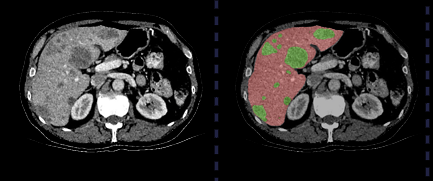
\includegraphics[scale=0.5]{images/imagerie.png}
\caption{Segmentation en imagerie médicale pour déceler des tumeurs}
\end{figure}

\begin{figure}[H]
\centering
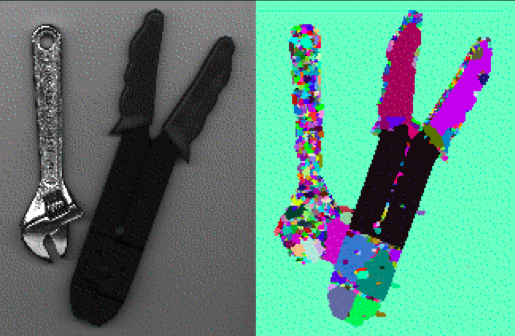
\includegraphics[scale=0.4]{images/segmentation.png}
\caption{Segmentation d'objets}
\end{figure}

\bigskip

L'homme sait naturellement séparer des objets dans une image, grâce à la compréhension des objets et de la scène,
mais la construction d'algorithme de segmentation de haut niveau représente un grand domaine de recherche dans le traitement d'image. 
Il existe 3 grandes classes de segmentation aujourd'hui :
\begin{itemize}
\item la segmentation fondée sur les régions,
\item la segmentation fondée sur les contours,
\item la segmentation fondée sur la classification/seuillage de pixels.
\end{itemize}

Dans ce projet, nous utilisons la méthode des contours avec le modèle de Mumford-Shah.
%Ce modèle a été implémenté par le groupe grâce à la plateforme GitHub. Le code source est disponible à cette adresse :
%{\small \url{à mettre }}.

